\documentclass[twocolumn,english]{article}
\usepackage[latin9]{inputenc}
\usepackage[landscape]{geometry}
\geometry{verbose,tmargin=0.5in,bmargin=0.75in,lmargin=0.5in,rmargin=0.5in}
\setlength{\parskip}{0bp}
\setlength{\parindent}{0pt}
\usepackage{color}
\usepackage{float}
\usepackage{amstext}
\usepackage{graphicx}
\PassOptionsToPackage{normalem}{ulem}
\usepackage{ulem}

\makeatletter



\usepackage{array}
\usepackage{multirow}
\usepackage{amsbsy}




\providecommand{\tabularnewline}{\\}

\setlength{\columnsep}{0.25in}
\usepackage{xcolor}
\usepackage{textcomp}
\usepackage{listings}
\lstset{
  tabsize=2,
  basicstyle=\small\ttfamily,
}



\usepackage{babel}
\usepackage{listings}
\renewcommand{\lstlistingname}{Listing}

\makeatother

\usepackage{babel}
\usepackage{listings}
\renewcommand{\lstlistingname}{Listing}

\begin{document}

\title{Reference Sheet for C220 Software Engineering Design}

\date{Autumn 2017}
\maketitle

\section{Test-Driven Development}

\paragraph{TDD Cycle}
\begin{enumerate}
\item Write a failing test (API design).
\item Code to pass test (internals design).
\item Refactor (structural design).
\end{enumerate}

\paragraph{Refactoring}

Process of improving the design of a piece of code, without changing
its functionality.
\begin{itemize}
\item Should be applied \emph{little and often} to continuously improve
design.
\item Only refactor in a \emph{green state}. Tests ensure that behaviour
is preserved.
\item Should be \emph{automated} to be done quickly and reliably.
\item Small transformations are \emph{combined} to achieve larger refactorings.
\end{itemize}

\paragraph{Example Transformations}
\begin{enumerate}
\item \emph{Compose (extract) method}: Break down method into chunks to
make it shorter. Allows us to give a name for a concept and increase
level of abstraction. Try to keep a constant level of abstraction.
\item \emph{Inline variable}: Instead of using a temporary variable, inline
its usages. Reduces number of elements in method.
\item \emph{Extract to common class}: First work to make duplication exactly
the same. Then refactor it, e.g. to another object. Reduces duplication.
\end{enumerate}

\paragraph{Technical Debt}

Features are been added quickly, in an inelegant way. When not fixed
quickly, \emph{technical debt} builds up.

\subsubsection*{JUnit and JMock}

\begin{lstlisting}[language=Java,basicstyle={\footnotesize\ttfamily},commentstyle={\color{gray}\itshape}]
public class TestObjectTest {
  // Set up mockery, constants, mock objects and tested object
  @Rule public JUnityRuleMockery context = new JUnitRuleMockery();

  final Order EXAMPLE_PARAM = new ...;

  CalledObject calledObject = context.mock(CalledObject.class);
  ...

  TestObject testObject = new TestObject(calledObject, ...)

  @Test
  public void doesSomethingSpecific() {
    // Set up local variables for exceptions / return values
    SomeException exception = new SomeException();

    // Set up expectations
    context.checking(new Expectations() {{
      // Ignore: ignoring / allowing
      ignoring(unimportantMockObject);
      allowing(someMockObject).someMethod(with(any(ParamType.class)));
                               will(throwException(exception));

      // Expect: exactly(n) / atLeast(n) / atMost(n)
      exactly(1).of(anotherMockObject).someOtherMethod(exception);
      exactly(1).of(anotherMockObject).anotherMethod(EXAMPLE_PARAM);
                                       will(returnValue(x));

      // Don't expect: never
      never(aDifferentMockObject).aDifferentMethod();
    }});
    
    // Set up triggers
    testObject.testedMethod(EXAMPLE_PARAM, ...);
    testObject.anotherTestedMethod();

    // Make assertions
    assertThat(testObject.getSomeValue(), is(x));
  }
}
\end{lstlisting}

\section{UML Diagrams}

\subsubsection*{UML Class Diagrams}

\begin{figure}[H]
\centering{}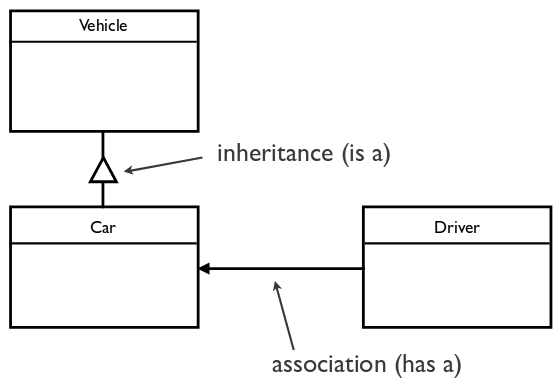
\includegraphics[width=0.35\columnwidth]{img/uml-class}
\end{figure}

\subsubsection*{UML Object Diagrams}

\begin{figure}[H]
\centering{}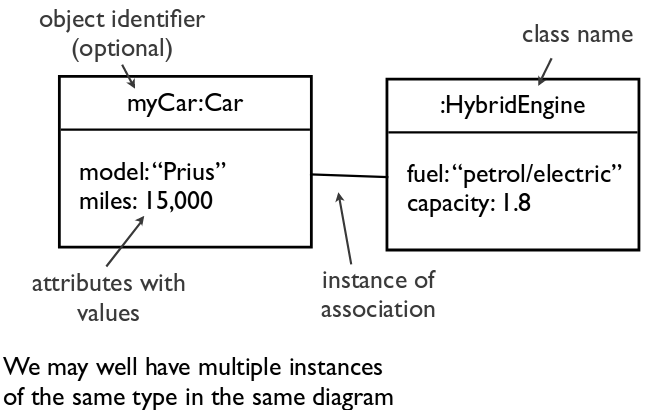
\includegraphics[width=0.4\columnwidth]{img/uml-object}
\end{figure}

\subsubsection*{UML Sequence Diagrams}

\begin{figure}[H]
\centering{}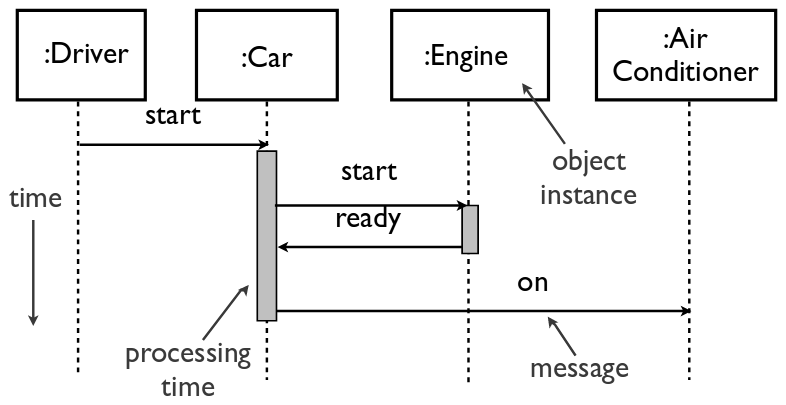
\includegraphics[width=0.5\columnwidth]{img/uml-sequence}
\end{figure}

\section{Object Oriented Design}

\paragraph{Four Elements of Simple Design}

In order of importance:
\begin{enumerate}
\item Behaves correctly.
\item Minimises duplication.
\item Maximises clarity.
\item Has fewer elements.
\end{enumerate}

\paragraph{Bad Design}
\begin{itemize}
\item \emph{Rigidity}: software is hard to change.
\item \emph{Fragility}: when we change one part, other parts break unexpectedly.
\item \emph{Immobility}: it is hard to reuse elements of the code in other
applications.
\end{itemize}

\paragraph{Commands vs. Queries}
\begin{itemize}
\item \emph{Commands}:\emph{ Ask another object to do something for us}.
Don't care how it's done, don't expect return value. Changes state
of invoked object.
\item \emph{Queries}:\emph{ Ask another object to tell us a value} (so we
can do something with it). Should return value, but not have side
effects on state of invoked object.
\end{itemize}

\paragraph{Tell Don't Ask}

Objects send messages, requesting actions, but do not expect return
values. Only queries return values.

\paragraph{Law of Demeter}

\emph{Only talk to your immediate friends}. Implementations that depend
on pieces of the system further away result in tight coupling.

Avoid \emph{train wrecks}: \texttt{getX().getY().getZ().doSomething()}.

\paragraph{Visibility}
\begin{itemize}
\item \emph{Encapsulation}: ensure object's behaviour is only affected through
its API. Implementation and state of objects should be encapsulated.
Reduces fragility.
\item \emph{Information hiding}: conceal how an object implements functionality.
Increases abstraction, chunking up program into concepts.
\end{itemize}
\emph{Key idea}: Make things \texttt{private} unless they should exposed
as an API for other objects (and generally avoid \texttt{protected}).

\paragraph{Coupling and Cohesion}
\begin{itemize}
\item \emph{Coupling}: How dependent two classes are towards each other.
Reducing coupling reduces fragility and allows reuse.
\item \emph{Cohesion}: An object should have one basic responsibility. Increasing
cohesion makes objects easier to reason about and reuse.
\end{itemize}

\section{Metrics}

\paragraph{Coupling}
\begin{itemize}
\item \emph{Afferent coupling}: How many other classes use (\uline{a}rrive
at) this class (measures \emph{responsibility}).
\item \emph{Efferent coupling}: How many classes are used by (\uline{e}xit)
this class (measures \emph{independence}).
\item \emph{Instability}: $\text{Ce}/\left(\text{Ce}+\text{Ca}\right)$.
Core parts should be stable. Parts at the edges, e.g. UI, don't need
to be.
\end{itemize}

\section{Design Patterns}

\subsection{Null Object Pattern}

\paragraph{Problem}

Checking for null is ugly.

\paragraph{Solution}

Use an interface and add a Null Object class that does nothing.

\subsubsection*{Example}

\begin{lstlisting}[language=Java,basicstyle={\footnotesize\ttfamily},commentstyle={\color{gray}\itshape}]
interface Track {
  public void play ();
}

class NullTrack implements Track {
  public void play () {
    // do nothing
  }
} 
\end{lstlisting}

\subsection{Template Method Pattern}

\paragraph{Problem}

Requirements change over time, sometimes we need to adapt a small
part of an algorithm.

\paragraph{Solution}

Extend via inheritance.

\subsubsection*{Example}

\begin{figure}[H]
\centering{}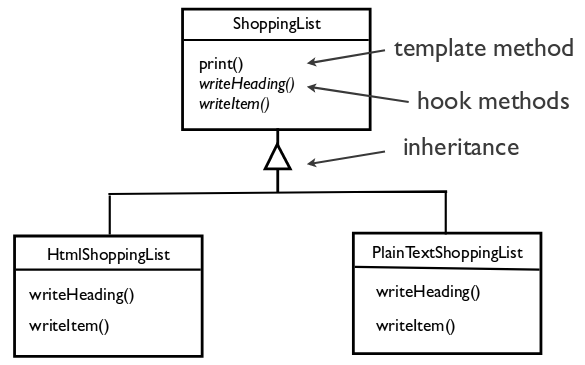
\includegraphics[width=0.5\columnwidth]{img/template-method}
\end{figure}

\paragraph{Benefits}
\begin{itemize}
\item Follows \emph{Hollywood Principle }(don't call us, we'll call you):
Concrete classes only define methods that are called when the superclass
needs them (they don't call up).
\item Follows \emph{Open-Closed Principle}: You should be able to extend
a class's behaviour without modifying it.
\begin{itemize}
\item Change behaviour by adding new code, rather than changing existing
code.
\item \emph{Separate things that change from things that stay the same}.
\end{itemize}
\end{itemize}

\paragraph{Drawbacks}

Immobility caused by coupling.

\subsection{Strategy Pattern}

\paragraph{Problem}

Requirements change over time, sometimes we need to adapt a small
part of an algorithm.

\paragraph{Solution}

Extend via delegation.

\subsubsection*{Example}

\begin{figure}[H]
\centering{}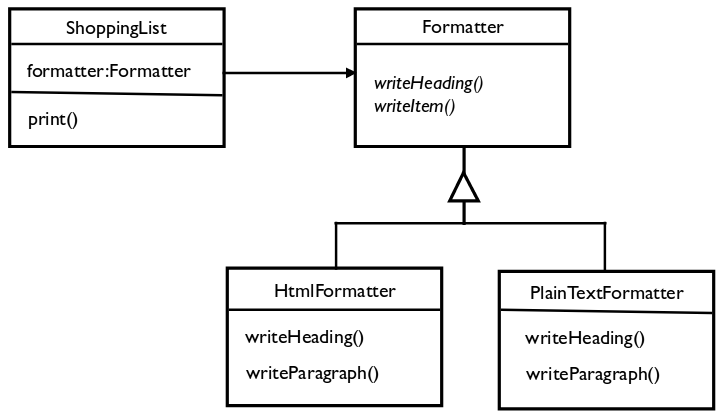
\includegraphics[width=0.6\columnwidth]{img/strategy}
\end{figure}

\paragraph{Benefits}

Does the same as the template method but with looser coupling.
\end{document}
